\subsection{Эллипс}
\textsl{Эллипс} --- плоская замкнутая кривая, сумма расстояний от любой точки котрой до двух фиксированных точек, называемых фокусами, постоянна и равна удвоенной большой полуоси эллипса.
\begin{equation}F_1M+F_2M=const=2a
\end{equation}
Главные отрезки эллипса:
\begin{enumerate}
\item Большая полуось ($a$)
\item Малая полуось ($b$)
\item Фокусное расстояние ($c$)
\end{enumerate}
$a$, $b$ и $c$ связаны слейдующим образом: $b^2+c^2=a^2$, что несложно вывести из определения эллипса.
 Эксцентриситет ($e$) --- числовая характеристика, показывающая степень отклонения от окружности. В эллипсе $0<e<1$.
 \begin{center}
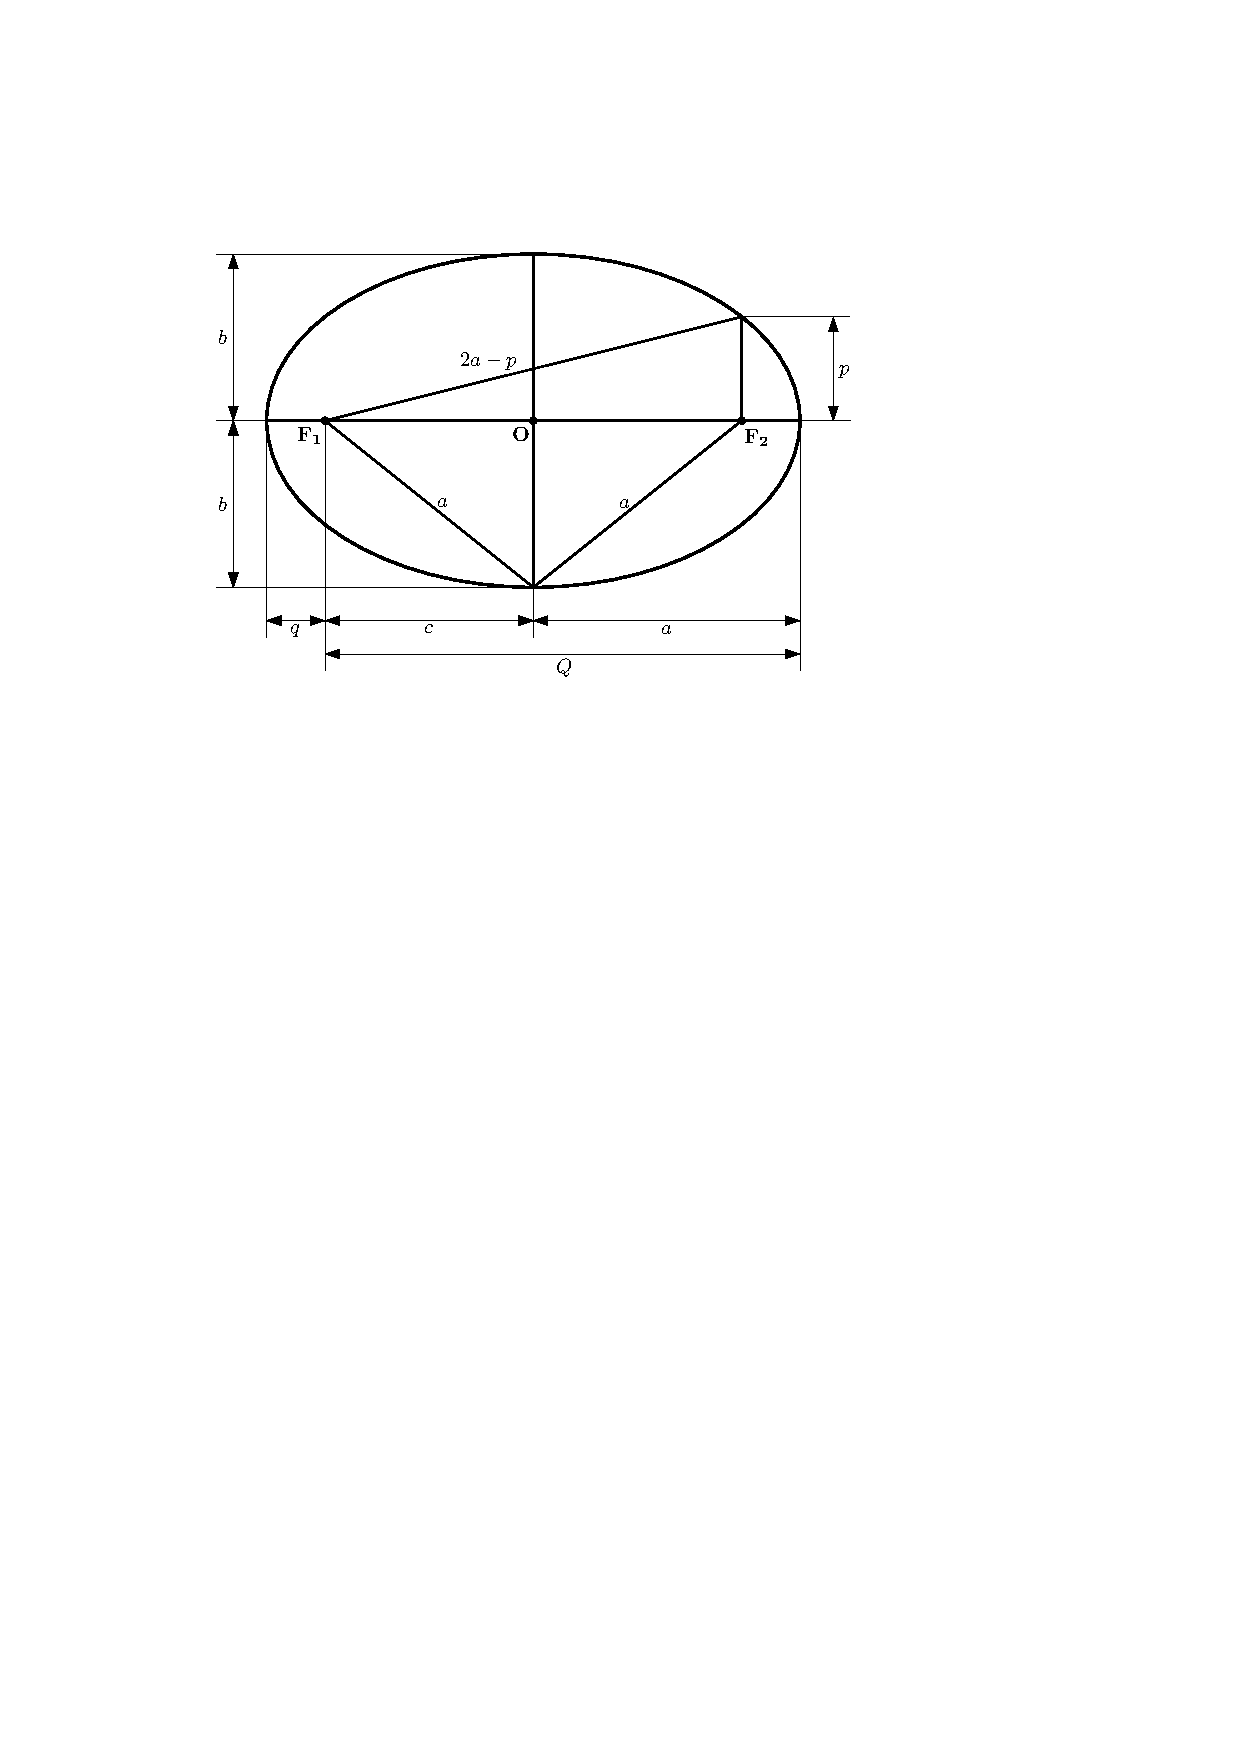
\includegraphics[width = 0.8\textwidth]{Ellips}
\begin{figure}[h!]
\caption{Эллипс}
\end{figure}
\end{center}
\textbf{Основные формулы для эллипса:}

Эксцетриситет
\begin{equation}
e=\frac{c}{a}=\sqrt{1-\frac{b^2}{a^2}}
\end{equation}

Расстояние до апоцентра
\begin{equation}
r_{\text{а}}=a(1+e)
\end{equation}

Расстояние до перицентра
\begin{equation}
r_{\text{п}}=a(1-e)
\end{equation}
Фокальный параметр

\begin{equation}
p=\frac{b^2}{a}=a(1-e^2)=b\sqrt{1-e^2}
\end{equation}
Площадь эллипса

\begin{equation}
S=\pi ab
\end{equation}

Радиус кривизны дуги эллипса в зависимости от расстояния $x$ от фокуса:
\begin{equation}
R=\frac{(2ax-x^2)^{3/2}}{ab}
\end{equation}
\begin{center}
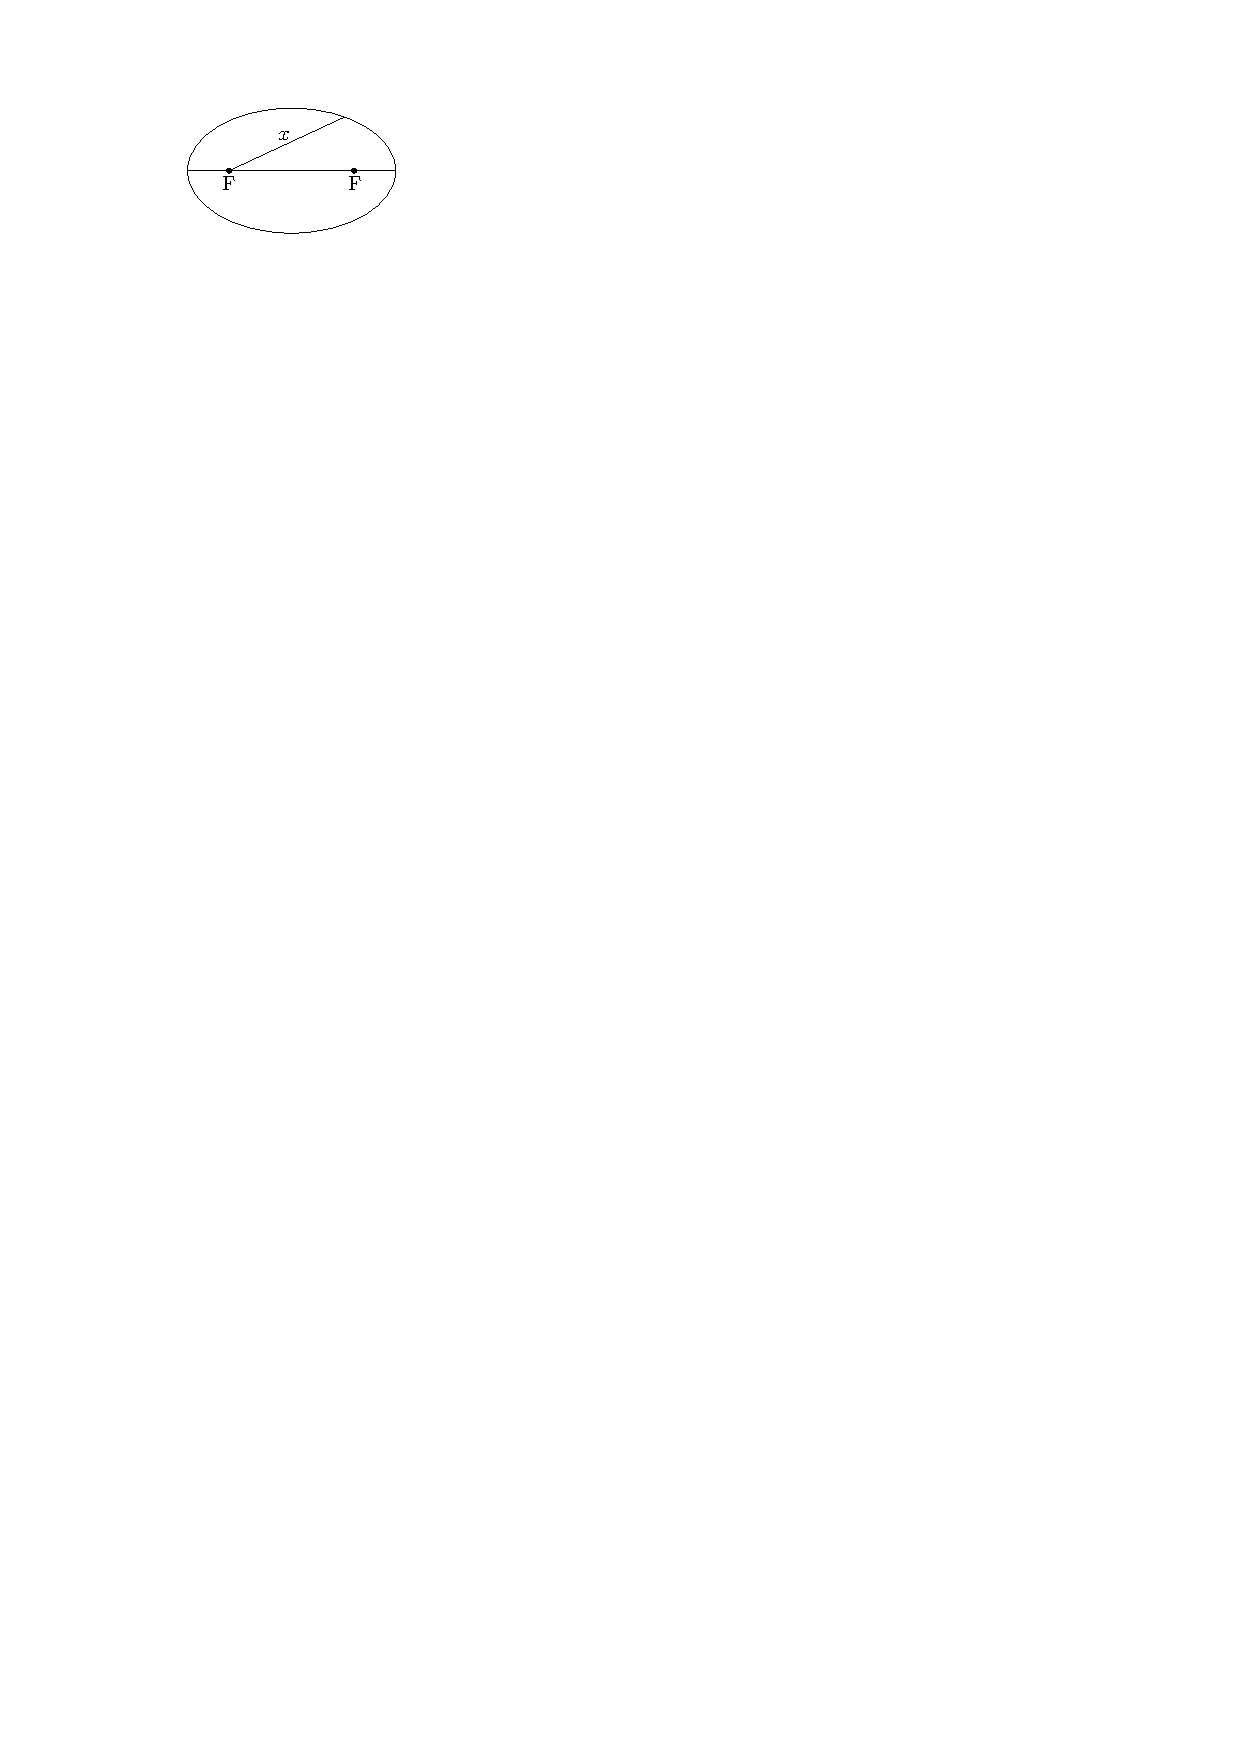
\includegraphics[width = 0.3\textwidth]{rad-curv}
\begin{figure}[!h]
\caption{К вычислению радиуса кривизны эллипса}
\end{figure}
\end{center}
\textbf{Уравнения эллипса:}

Каноническое уравнение
\begin{equation}
\frac{x^2}{a^2}+\frac{y^2}{b^2}=1
\end{equation}
Параметрическое уравнение
\begin{equation}
\left\{
\begin{aligned}
x=a\cos \phi\\
y=b\sin\phi\\
\end{aligned}
\right.
\end{equation}

Уравнение в полярных координатах, где $\phi$ --- истинная аномалия. При положительном знаке перед $e$ второй фокус эллипса будет находится в точке (0,2с), а при отрицательном --- в точке ($\pi$,2с).
\begin{equation}
r=\frac{p}{1\pm e\cos\phi}
\end{equation}

\textbf{Оптические свойства эллипса:}
\begin{enumerate}
\item Свет от источника, находящегося в одном из фокусов, отражается эллипсом так, что отражённые лучи пересекутся во втором фокусе.
\item Свет от источника, находящегося в одном из фокусов, отражается эллипсом так, что отражённые лучи ни в каком фокусе не пересекутся.
\end{enumerate}





 
